\documentclass[12pt, letterpaper]{article}

\usepackage{amsmath} % For mathematical symbols and environments
\usepackage{fullpage}
\usepackage{amsfonts, amssymb}

\usepackage[top=1in, bottom=1in, left=1in, right=0.75in, paperwidth=8.5in, paperheight=10in ]{geometry}

\usepackage{amsfonts} % for specialized math notations

% Macros for defining custom latex commands. Used as a function.
\def\eq1{$y = \frac{5x}{3x^2+3x+3}$}

\usepackage{float}
\usepackage{tikz, pgfplots}
% for images
\usepackage{graphicx}
\begin{document}
	\begin{figure}[H]
		\centering
		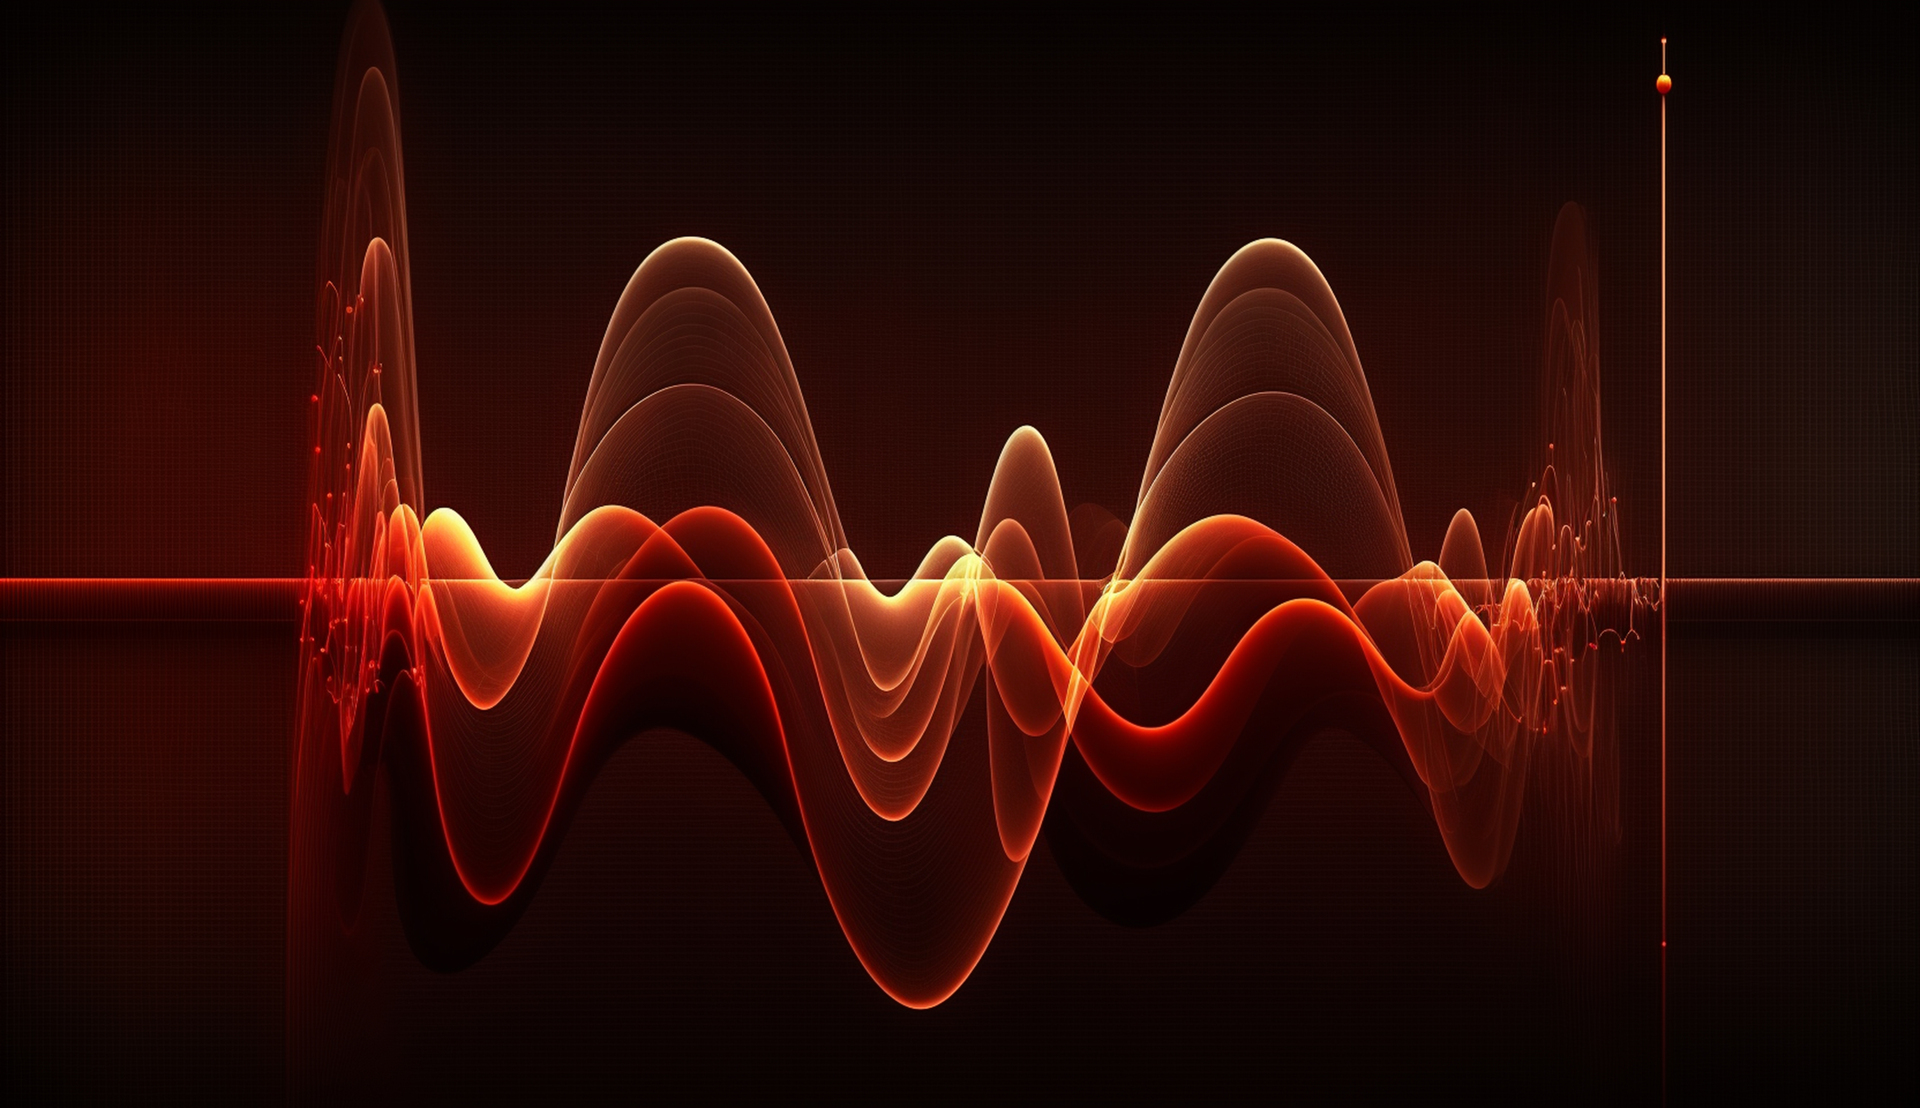
\includegraphics[scale=0.8]{simple}
		\caption{Random Text}
	\end{figure}
	
	\section*{Short Questions}
	
	\begin{enumerate}
		\item Using function declares above \eq1
		\item Simplify: $ \frac{2x^2 + 4x}{x} $
		\item This is symbol for all real number : $\mathbb{R}$ and set of all integers: $\mathbb{Z}$.
		\item This is symbol for all rational number : $\mathbb{Q}$
		
		\item Solve for $x$: $ 3x + 5 = 11 $
		\item Differentiate: $ f(x) = 5x^3 + 2x^2 - x + 7 $
		\item Evaluate: $ \int_0^1 (2x + 1) \, dx $
		\item Expand: $ (a + b)^3 $
	\end{enumerate}
	
\end{document}\\
